\documentclass[11pt,a4paper]{article}
\usepackage[utf8]{inputenc}
\usepackage{amsmath}
\usepackage{tikz}
\usetikzlibrary{shapes,arrows,positioning,fit,backgrounds,decorations.pathreplacing,calc}
\usepackage{geometry}
\geometry{margin=1in}

\title{Brain-to-Text Model Architectures}
\author{Brain-to-Text Competition}
\date{}

\begin{document}

\maketitle

\section{Baseline CTC Architecture}

\begin{figure}[h]
\centering
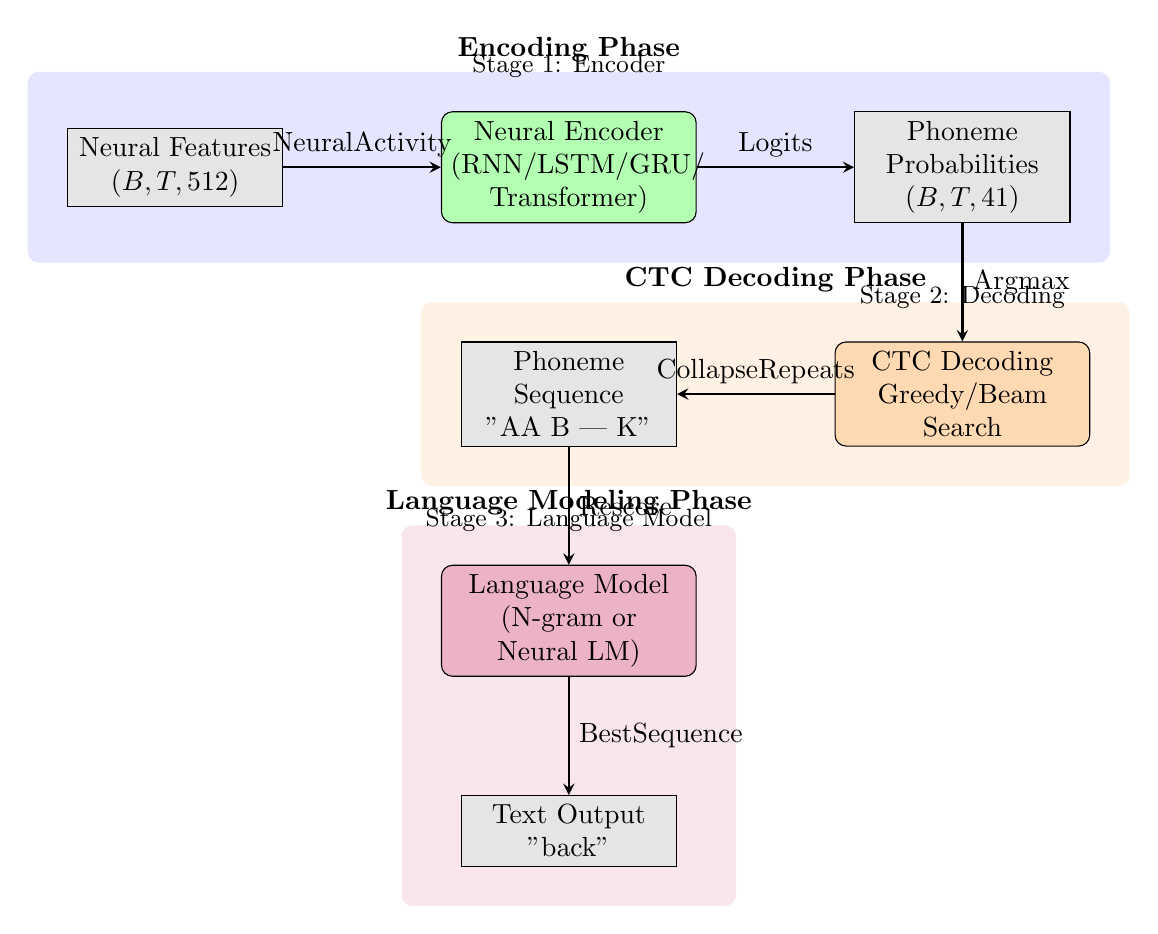
\begin{tikzpicture}[
    node distance=1.5cm and 2cm,
    block/.style={rectangle, draw, fill=blue!20, text width=3cm, text centered, rounded corners, minimum height=1cm},
    encoder/.style={rectangle, draw, fill=green!30, text width=3cm, text centered, rounded corners, minimum height=1cm},
    decoder/.style={rectangle, draw, fill=orange!30, text width=3cm, text centered, rounded corners, minimum height=1cm},
    lm/.style={rectangle, draw, fill=purple!30, text width=3cm, text centered, rounded corners, minimum height=1cm},
    data/.style={rectangle, draw, fill=gray!20, text width=2.5cm, text centered, minimum height=0.8cm},
    arrow/.style={->, >=stealth, thick}
]

% Input
\node[data] (input) {Neural Features\\$(B, T, 512)$};

% Encoder
\node[encoder, right=of input] (encoder) {Neural Encoder\\(RNN/LSTM/GRU/\\Transformer)};

% Phoneme probabilities
\node[data, right=of encoder] (phoneme_probs) {Phoneme\\Probabilities\\$(B, T, 41)$};

% CTC Decoding
\node[decoder, below=of phoneme_probs] (ctc_decode) {CTC Decoding\\Greedy/Beam\\Search};

% Phoneme sequence
\node[data, left=of ctc_decode] (phonemes) {Phoneme\\Sequence\\"AA B | K"};

% Language Model
\node[lm, below=of phonemes] (lm) {Language Model\\(N-gram or\\Neural LM)};

% Output
\node[data, below=of lm] (output) {Text Output\\"back"};

% Arrows
\draw[arrow] (input) -- (encoder) node[midway, above] {Neural\\Activity};
\draw[arrow] (encoder) -- (phoneme_probs) node[midway, above] {Logits};
\draw[arrow] (phoneme_probs) -- (ctc_decode) node[midway, right] {Argmax};
\draw[arrow] (ctc_decode) -- (phonemes) node[midway, above] {Collapse\\Repeats};
\draw[arrow] (phonemes) -- (lm) node[midway, right] {Rescore};
\draw[arrow] (lm) -- (output) node[midway, right] {Best\\Sequence};

% Annotations
\node[above=0.3cm of encoder, font=\small] {Stage 1: Encoder};
\node[above=0.3cm of ctc_decode, font=\small] {Stage 2: Decoding};
\node[above=0.3cm of lm, font=\small] {Stage 3: Language Model};

% Details box
\begin{scope}[on background layer]
    \node[fill=blue!10, rounded corners, fit=(input)(encoder)(phoneme_probs), inner sep=0.5cm, label=above:\textbf{Encoding Phase}] {};
    \node[fill=orange!10, rounded corners, fit=(ctc_decode)(phonemes), inner sep=0.5cm, label=above:\textbf{CTC Decoding Phase}] {};
    \node[fill=purple!10, rounded corners, fit=(lm)(output), inner sep=0.5cm, label=above:\textbf{Language Modeling Phase}] {};
\end{scope}

\end{tikzpicture}
\caption{Baseline CTC Architecture: Two-stage approach converting neural features to phonemes, then phonemes to text using a language model.}
\label{fig:ctc_arch}
\end{figure}

\subsection{CTC Architecture Details}

The baseline CTC architecture consists of three main stages:

\begin{enumerate}
    \item \textbf{Encoding}: Neural features (512 channels, variable length $T$) are processed by an encoder (RNN, LSTM, GRU, or Transformer) to produce phoneme probabilities at each timestep. Output shape: $(B, T, 41)$ where 41 = 40 phonemes + 1 blank token.
    
    \item \textbf{CTC Decoding}: Phoneme probabilities are decoded using CTC algorithm:
    \begin{itemize}
        \item Greedy: Take most likely phoneme at each timestep
        \item Collapse consecutive repeats
        \item Remove blank tokens
        \item Result: Phoneme sequence (e.g., "AA B | K")
    \end{itemize}
    
    \item \textbf{Language Modeling}: Phoneme sequence is converted to text using a language model:
    \begin{itemize}
        \item N-gram models (1-gram, 3-gram, 5-gram)
        \item Neural language models (GPT-2, BERT)
        \item Rescores multiple hypotheses to find best text
        \item Result: Final text output (e.g., "back")
    \end{itemize}
\end{enumerate}

\vspace{1cm}

\section{End-to-End (E2E) Architecture}

\begin{figure}[h]
\centering
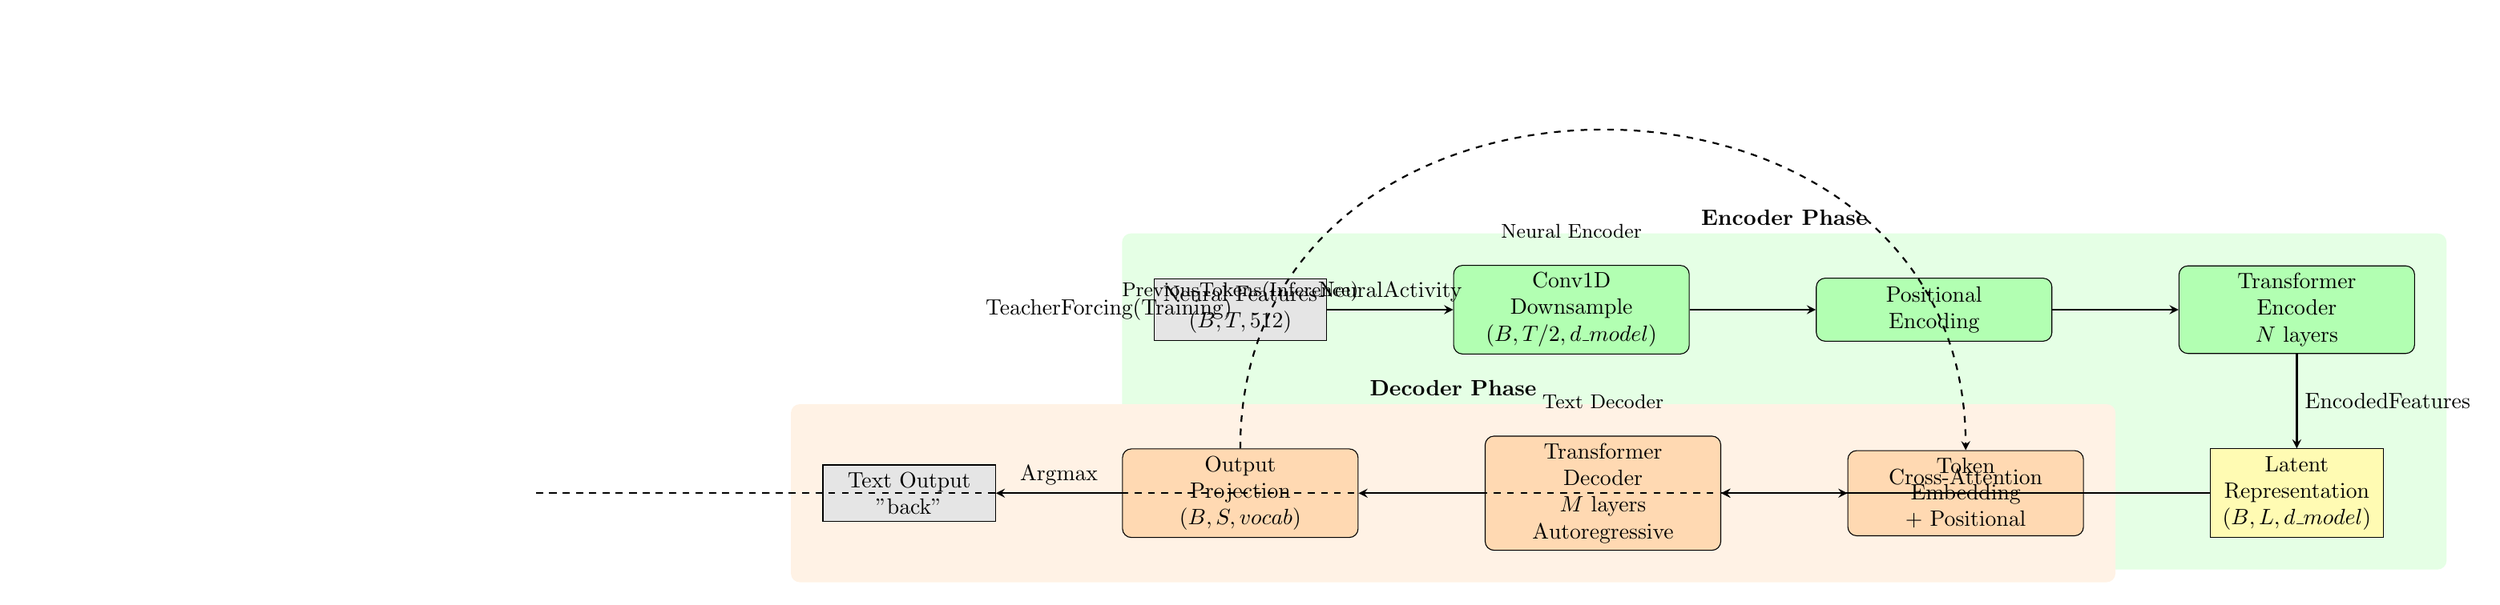
\begin{tikzpicture}[
    node distance=1.5cm and 2cm,
    block/.style={rectangle, draw, fill=blue!20, text width=3cm, text centered, rounded corners, minimum height=1cm},
    encoder/.style={rectangle, draw, fill=green!30, text width=3.5cm, text centered, rounded corners, minimum height=1cm},
    decoder/.style={rectangle, draw, fill=orange!30, text width=3.5cm, text centered, rounded corners, minimum height=1cm},
    data/.style={rectangle, draw, fill=gray!20, text width=2.5cm, text centered, minimum height=0.8cm},
    latent/.style={rectangle, draw, fill=yellow!30, text width=2.5cm, text centered, minimum height=0.8cm},
    arrow/.style={->, >=stealth, thick},
    dashed_arrow/.style={->, >=stealth, thick, dashed}
]

% Input
\node[data] (input) {Neural Features\\$(B, T, 512)$};

% Conv projection
\node[encoder, right=of input] (conv_proj) {Conv1D\\Downsample\\$(B, T/2, d\_model)$};

% Positional encoding
\node[encoder, right=of conv_proj] (pos_enc) {Positional\\Encoding};

% Transformer encoder
\node[encoder, right=of pos_enc] (transformer_enc) {Transformer\\Encoder\\$N$ layers};

% Latent representation
\node[latent, below=of transformer_enc] (latent) {Latent\\Representation\\$(B, L, d\_model)$};

% Token embedding
\node[decoder, left=of latent] (token_emb) {Token\\Embedding\\+ Positional};

% Transformer decoder
\node[decoder, left=of token_emb] (transformer_dec) {Transformer\\Decoder\\$M$ layers\\Autoregressive};

% Output projection
\node[decoder, left=of transformer_dec] (output_proj) {Output\\Projection\\$(B, S, vocab)$};

% Output
\node[data, left=of output_proj] (output) {Text Output\\"back"};

% Arrows - Encoder path
\draw[arrow] (input) -- (conv_proj) node[midway, above] {Neural\\Activity};
\draw[arrow] (conv_proj) -- (pos_enc);
\draw[arrow] (pos_enc) -- (transformer_enc);
\draw[arrow] (transformer_enc) -- (latent) node[midway, right] {Encoded\\Features};

% Arrows - Decoder path
\draw[arrow] (latent) -- (transformer_dec) node[midway, above] {Cross-\\Attention};
\draw[arrow] (token_emb) -- (transformer_dec);
\draw[arrow] (transformer_dec) -- (output_proj);
\draw[arrow] (output_proj) -- (output) node[midway, above] {Argmax};

% Teacher forcing arrow (dashed)
\draw[dashed_arrow] (output) to[out=180, in=180, looseness=2] (token_emb) node[midway, left] {Teacher\\Forcing\\(Training)};

% Autoregressive arrow (dashed)
\draw[dashed_arrow] (output_proj) to[out=90, in=90, looseness=1.5] (token_emb) node[midway, above, font=\small] {Previous\\Tokens\\(Inference)};

% Annotations
\node[above=0.3cm of conv_proj, font=\small] {Neural Encoder};
\node[above=0.3cm of transformer_dec, font=\small] {Text Decoder};

% Details box
\begin{scope}[on background layer]
    \node[fill=green!10, rounded corners, fit=(input)(conv_proj)(pos_enc)(transformer_enc)(latent), inner sep=0.5cm, label=above:\textbf{Encoder Phase}] {};
    \node[fill=orange!10, rounded corners, fit=(token_emb)(transformer_dec)(output_proj)(output), inner sep=0.5cm, label=above:\textbf{Decoder Phase}] {};
\end{scope}

\end{tikzpicture}
\caption{End-to-End Architecture: Direct mapping from neural features to text without intermediate phoneme representation.}
\label{fig:e2e_arch}
\end{figure}

\subsection{E2E Architecture Details}

The end-to-end architecture consists of two main components:

\begin{enumerate}
    \item \textbf{Neural Encoder}:
    \begin{itemize}
        \item \textbf{Convolutional Projection}: Downsamples neural features from $(B, T, 512)$ to $(B, T/2, d\_model)$ using Conv1D with stride 2
        \item \textbf{Positional Encoding}: Adds sinusoidal positional encodings to preserve temporal information
        \item \textbf{Transformer Encoder}: $N$ layers of self-attention and feed-forward networks
        \item \textbf{Output}: Latent representation $(B, L, d\_model)$ where $L = T/2$
    \end{itemize}
    
    \item \textbf{Text Decoder}:
    \begin{itemize}
        \item \textbf{Token Embedding}: Converts character/token IDs to embeddings with positional encoding
        \item \textbf{Transformer Decoder}: $M$ layers with:
        \begin{itemize}
            \item Self-attention (causal mask for autoregressive generation)
            \item Cross-attention to encoder output
            \item Feed-forward networks
        \end{itemize}
        \item \textbf{Output Projection}: Maps decoder output to vocabulary logits $(B, S, vocab\_size)$
        \item \textbf{Generation}: 
        \begin{itemize}
            \item Training: Teacher forcing (uses ground truth tokens)
            \item Inference: Autoregressive (uses previously generated tokens)
        \end{itemize}
    \end{itemize}
\end{enumerate}

\subsection{Key Differences from CTC}

\begin{itemize}
    \item \textbf{No Phoneme Intermediate}: Directly maps neural features to text characters/tokens
    \item \textbf{Single Objective}: Cross-entropy loss for next-token prediction
    \item \textbf{Autoregressive}: Generates text one token at a time
    \item \textbf{No Language Model}: Language modeling is learned implicitly in the decoder
    \item \textbf{End-to-End Optimization}: All components trained jointly
\end{itemize}

\section{Comparison}

\begin{table}[h]
\centering
\begin{tabular}{|l|p{6cm}|p{6cm}|}
\hline
\textbf{Aspect} & \textbf{CTC Architecture} & \textbf{E2E Architecture} \\
\hline
\textbf{Stages} & 3 (Encoder, CTC Decode, LM) & 2 (Encoder, Decoder) \\
\hline
\textbf{Intermediate} & Phonemes & Latent representation \\
\hline
\textbf{Loss Function} & CTC Loss & Cross-Entropy Loss \\
\hline
\textbf{Decoding} & Parallel (all timesteps) & Sequential (autoregressive) \\
\hline
\textbf{Language Model} & Required (external) & Learned (implicit) \\
\hline
\textbf{Training Speed} & Faster (parallel) & Slower (autoregressive) \\
\hline
\textbf{Interpretability} & High (phonemes visible) & Lower (black box) \\
\hline
\textbf{Data Requirements} & Moderate & Higher \\
\hline
\end{tabular}
\caption{Comparison between CTC and E2E architectures}
\label{tab:comparison}
\end{table}

\end{document}

